
\documentclass{beamer}
\usetheme{Boadilla}
\usepackage{amsfonts,amsmath,amssymb}
\usepackage{dsfont,fontawesome}
\usepackage{braket,mathtools,siunitx}
\usepackage{hyperref}
\usepackage{textcomp,url}
\usepackage{graphicx}
\usepackage{listings,enumerate}
\usepackage{booktabs,tabularx,longtable,multicol}
\usepackage{subcaption}
% If I can ever figure out embedding videos
%%\usepackage{media9}
%%\usepackage{multimedia}

\lstset{language=C}

\setbeamercovered{transparent}


\newcommand*\limitset[1]{{#1}^\prime}
% Not working in unicode math with xelatex for some reason...
% \newcommand*\closure[1]{\overline #1}
\newcommand*\closureunion[1]{{#1}\cup \limitset{#1}}
\newcommand*\interior[1]{{#1}^\circ}

% Sets of points
% The set of points within some distance #1 from #2
\newcommand*\neighbor[2]{N_{#1}({#2})}
% The neighborhood without #2
\newcommand*\delneighbor[2]{N_{#1}^*({#2})}
\newcommand*\conjugate[1]{\overline{#1}}
\newcommand*\sequence[2]{\set{#1}_{#2=1}^\infty}
\newcommand*\series[2]{\sum_{#2=1}^\infty #1_{#2}}
\newcommand*\compose[2]{#1 \circ #2}
\newcommand*\udisk{\mathbb{D}}
\newcommand*\disk[2]{D_{#1}(#2)}
\newcommand*\punctdisk[2]{\disk_{ #1 } - \set{#2}}
\newcommand*\complex{\mathbb{C}}
\newcommand*\naturals{\mathbb{N}}
\newcommand{\integers}{\mathbb{Z}}
\newcommand*\rationals{\mathbb{Q}}
\newcommand*\reals{\mathbb{R}}

% Function spaces
\newcommand*\cnfunc[2]{C^{#2}\left(#1 \right)}
\newcommand*\cnfuncdom[1]{C^{#1}\left(\domain \right)}
\newcommand*\linffunc[1]{L^{\infty}\left(#1 \right)}
\newcommand*\linffuncdom{L^{\infty}\left(\domain \right)}
\newcommand*\lnfunc[2]{L^{#2}\left(#1 \right)}
\newcommand*\lnfuncdom[1]{L^{#1}\left(\domain \right)}
\newcommand*\sobolev[3]{W^{#2, #3}\left(#1 \right)}
\newcommand*\sobolevdom[2]{W^{#1, #2}\left(\domain \right)}
\newcommand*\sobolevh[2]{H^{#2}\left(#1 \right)}
\newcommand*\sobolevhdom[1]{H^{#1}\left(\domain \right)}
\newcommand*\sobolevcs[3]{W_0^{#2, #3}\left(#1 \right)}
\newcommand*\sobolevcsdom[2]{W_0^{#1, #2}\left(\domain \right)}
\newcommand*\sobolevhcs[2]{H_0^{#2}\left(#1 \right)}
\newcommand*\sobolevhcsdom[1]{H_0^{#1}\left(\domain \right)}

\newcommand*\grad{D}
\newcommand*\graddir[1]{D_{#1}}
\newcommand*\lapl{∆}
\newcommand*\diffquot[1]{D^{#1}}
\newcommand*\diffquotdir[2]{D_{#2}^{#1}}

\newcommand*\domain{U}
\newcommand*\bndry[1]{\partial #1}
\newcommand*\bndrydom{\partial \domain}
\newcommand*\compactcont{\subset \subset} % U \compactcont V \rightarrow U \subset \closure{U} \subset V, where U, V are (open) domains

\newcommand*\ballunit{B_1}
\newcommand*\ball[2]{B_{#2}(#1)}
\newcommand*\bunitsurfarea[1]{\omega_{#1}}
\newcommand*\bunitsurfareadef{\omega_n}
\newcommand*\bunitvolume[1]{\alpha_{#1}}
\newcommand*\bunitvolumedef{\alpha_n}

% Limit
\newcommand*\limitto[2]{\lim \limits_{#1 \rightarrow #2}}

% Partial Derivatives
\newcommand{\dd}[1]{\;\mathrm{d}#1}
\newcommand{\dx}{\dd{x}}
\newcommand{\dy}{\dd{y}}
\newcommand{\dz}{\dd{z}}
\newcommand{\dr}{\dd{r}}
\newcommand{\ds}{\dd{s}}
\newcommand{\dS}{\dd{S}}
\newcommand{\dt}{\dd{t}}
\newcommand*\pderiv[2]{\frac{\partial #1}{\partial #2}}
\newcommand*\nthpderiv[3]{\frac{\partial^{#3} #1}{\partial #2^{#3}}}
\newcommand*\deriv[2]{\frac{\dd{#1}}{\dd{#2}}}
\newcommand*\nthderiv[3]{\frac{\dd{^{#3} #1}}{\dd{#2^{#3}}}}

% Mesh and Metric variable aliases
\newcommand*{\complexity}{\mathcal{C}}
\newcommand*{\mtensor}{\mathcal{M}}

% Norms
\newcommand*\linfnorm[2]{\left\lVert#1\right\rVert_{L^{\infty}(#2)}}
\newcommand*\linfnormdom[1]{\left\lVert#1\right\rVert_{L^{\infty}(\domain)}}

\newcommand*\lnorm[3]{\left\lVert#1\right\rVert_{L^{#2}(#3)}}
\newcommand*\lnormdom[2]{\left\lVert#1\right\rVert_{L^{#2}(\domain)}}

\newcommand*\hnorm[3]{\left\lVert#1\right\rVert_{H^{#2}(#3)}}
\newcommand*\hnormdom[2]{\left\lVert#1\right\rVert_{H^{#2}(\domain)}}

\newcommand*\wnorm[4]{\left\lVert#1\right\rVert_{W^{#2, #3}(#4)}}
\newcommand*\wnormdom[3]{\left\lVert#1\right\rVert_{W^{#2, #3}(\domain)}}

\newcommand*\vecnorm[1]{\left\lVert#1\right\rVert}

\DeclareMathOperator{\res}{res}
\DeclareMathOperator{\sign}{sign}
\DeclareMathOperator{\diam}{diam}
\DeclareMathOperator{\partition}{Partition}
\DeclareMathOperator{\Area}{Area}

% Matrix computations
\newcommand*\trace[1]{\text{tr}\left( #1 \right)}

% Average integral from https://tex.stackexchange.com/questions/759/average-integral-symbol
\def\Xint#1{\mathchoice
{\XXint\displaystyle\textstyle{#1}}%
{\XXint\textstyle\scriptstyle{#1}}%
{\XXint\scriptstyle\scriptscriptstyle{#1}}%
{\XXint\scriptscriptstyle\scriptscriptstyle{#1}}%
\!\int}
\def\XXint#1#2#3{{\setbox0=\hbox{$#1{#2#3}{\int}$ }
\vcenter{\hbox{$#2#3$ }}\kern-.6\wd0}}
\def\ddashint{\Xint=}
\def\dashint{\Xint-}
\def\avgint{\dashint}


\title{C++ Standard Library}

\begin{document}

\begin{frame}
  \titlepage
\end{frame}

\begin{frame}
  \frametitle{The Standard Library}
  is huge:
  \begin{itemize}
    \item {\bf Containers library}
    \item {\bf Algorithms library}
    \item {\bf Numerics library}
    \item Ranges library (C++20)
    \item Concepts library (C++20)
    \item Atomic operations library (C++11)
    \item Utilities library
    \item Iterators library
    \item Thread support library (C++11)
    \item Input/output library
    \item Diagnostics library
    \item Strings library
    \item Localizations library
    \item Filesystem library (C++17)
    \item Regular expressions library (C++11)
  \end{itemize}
\end{frame}

\begin{frame}
  \frametitle{Containers Library}
  Many containers are provided, these are the most commonly used
  \begin{itemize}
    \item array
    \item vector
    \item set (and unordered\_set)
    \item map (and unordered\_map)
  \end{itemize}
\end{frame}

\begin{frame}
  \frametitle{std::array}
  \begin{itemize}
  \item Statically allocated array of objects
  \item Access time: $O(1)$
  \item Size must be known at compile time
  \item Contained objects must be default constructible
  \item Primitive types need to be manually initialized
  \end{itemize}
  Why use this instead of a C array?
  \begin{itemize}
  \item Automatic and correct pairing of the array and its size
    - if an std::array is passed as a parameter, you know how large it is, unlike with a C array
  \item Compatibility with for each loop syntax and standard algorithms
  \item Bounds checking with .at
  \end{itemize}
\end{frame}

\begin{frame}
  \frametitle{std::vector}
  \begin{itemize}
  \item Resizable array of objects
  \item Access time: $O(1)$
  \item Insertion time: $O(n)$
  \item Append time: $O(1)$ amortized; with an upper bound of $O(n)$
  \item Search time: $O(n)$
  \end{itemize}
\end{frame}

\begin{frame}
  \frametitle{map and set datastructure}
  \begin{itemize}
  \item map and set maintain a sorted collection of data
    - storing the data in a vector or array would be really inefficient
  \item std::set is a collection of unique objects - inserting an already contained element has no effect
  \item std::map associates keys with values
  \item Most C++ standard library implementations use a red-black tree instead
  \item Red-black trees are self-balancing binary trees with the following time complexities:
    \begin{itemize}
    \item Insert - $O(\log(n))$
    \item Delete - $O(\log(n))$
    \item Search - $O(\log(n))$
    \end{itemize}
  \end{itemize}
\end{frame}

\begin{frame}
  \frametitle{Balanced Binary Tree}
  Balanced binary trees are trees with the difference in heights of the left and right subtrees
  of the root being at most 1.
  \begin{figure}[ht]
    \begin{multicols}{3}
      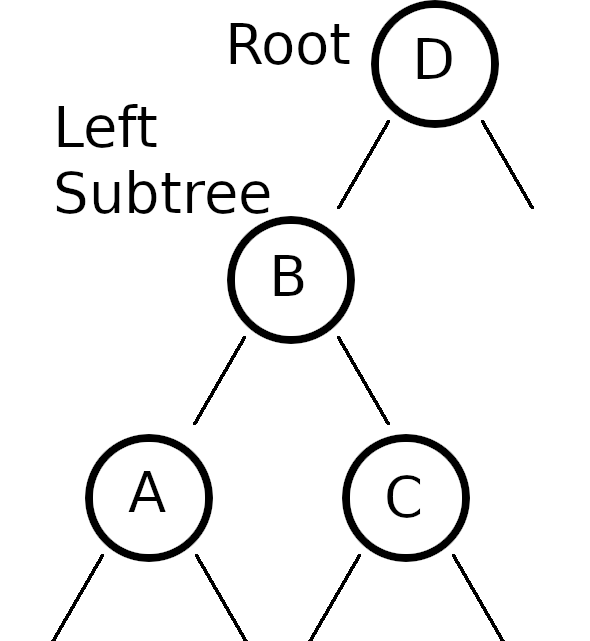
\includegraphics[width=0.25\textwidth]{figures/unbalanced_binary_tree.png}
      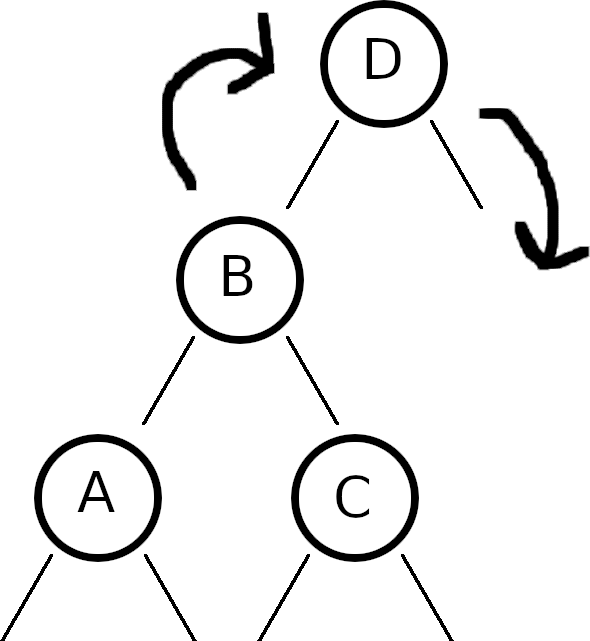
\includegraphics[width=0.25\textwidth]{figures/unbalanced_binary_tree_rotation.png}
      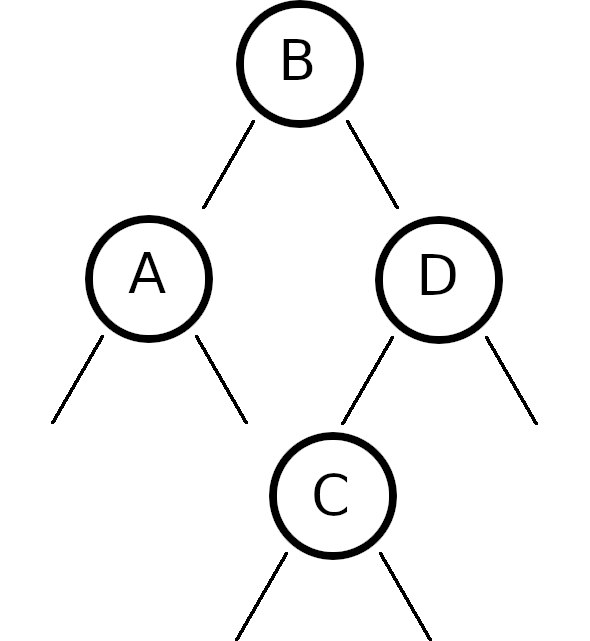
\includegraphics[width=0.25\textwidth]{figures/balanced_binary_tree.png}
    \end{multicols}
    \caption{Binary trees - {\bf Left}: Unbalanced tree, {\bf Center}: Rebalancing rotation,
      {\bf Right}: Balanced tree}
  \end{figure}
  Rebalancing nearly balanced binary trees is a constant time operation
\end{frame}

\begin{frame}
  \frametitle{unordered\_map and unordered\_set datastructures}
  The unordered versions of map and set use a hash map with buckets to store their data.
  \begin{figure}[ht]
    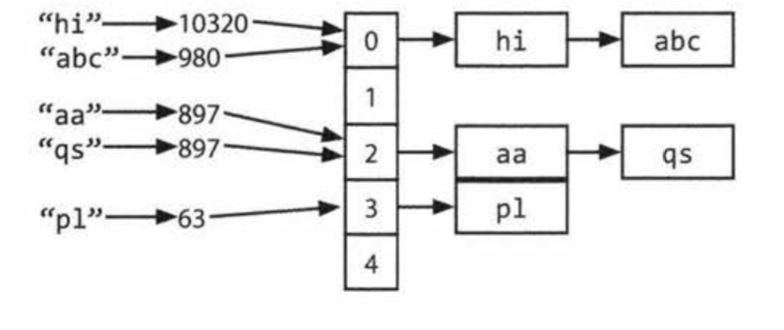
\includegraphics[width=0.8\textwidth]{figures/hash_map_buckets.png}
    \caption{Hash map example {\tiny (source: https://blog.miyozinc.com/algorithms/custom-hashmap-implementation-in-java/)}}
  \end{figure}
\end{frame}

\begin{frame}
  \frametitle{unordered\_map and unordered\_set datastructures}
  Time complexities (using a vector for each bucket):
  \begin{itemize}
    \item Insert: $O(1)$
    \item Delete: $O(n)$
    \item Search: $O(n)$
  \end{itemize}
  Not really convincing... With rare hash collisions we get instead
  \begin{itemize}
    \item Insert: $O(1)$
    \item Delete: $O(1)$
    \item Search: $O(1)$
  \end{itemize}

\end{frame}

\begin{frame}
  \frametitle{Algorithms Library}
  A more complete and in depth overview: https://youtu.be/2olsGf6JIkU
  \begin{itemize}
    \item {\bf sort, stable\_sort}
    \item {\bf find, find\_if, find\_if\_not}
    \item {\bf transform}
    \item {\bf accumulate, reduce}
    \item {\bf partial\_sum, exclusive\_scan, inclusive\_scan}
    \item {\bf set\_intersection, set\_union, set\_difference, set\_symmetric\_difference}
    \item for\_each
    \item copy, copy\_if
    \item unique
    \item reverse
    \item rotate
    \item is\_permutation
    \item next\_permutation, prev\_permutation
    \item all\_of, any\_of, none\_of
    \item ...
  \end{itemize}
\end{frame}

\begin{frame}[fragile]
  \frametitle{sort, stable\_sort}
  Efficient sorting algorithm, std::sort has:\\
  $O(n \log(n))$ time complexity\\
  $O(\log(n))$ extra space complexity\\
  Usage:
  \begin{lstlisting}[language=C++]
  // MyType has `bool operator<(const MyType &rhs)`
  std::vector<MyType> my_vec = ...;
  std::sort(my_vec.begin(), my_vec.end());

  // Alternatively, define
  bool compare_my_type(const MyType &lhs,
                       const MyType &rhs) { ... }
  // and then
  std::sort(my_vec.begin(), my_vec.end(),
            compare_my_type);
  \end{lstlisting}
\end{frame}

\begin{frame}[fragile]
  \frametitle{find, find\_if, find\_if\_not}
  Searches a collection for a specific value, or one that satisfies a predicate:\\
  $O(n)$ time complexity\\
  Usage:
  \begin{lstlisting}[language=C++]
std::vector<MyType> vec = {...};
auto itr = std::find(vec.begin(), vec.end(),
  my_value);

// Or with the predicate:
bool predicate(const MyType &val);
auto itr = std::find_if(vec.begin(), vec.end(),
  predicate);
// Negating the predicate
auto itr = std::find_if_not(vec.begin(),
  vec.end(), predicate);
  \end{lstlisting}
\end{frame}

\begin{frame}[fragile]
  \frametitle{transform}
  Applies a function to each element of the container,
  storing the result in another container of the same size.
  Additionally provides a version which takes pairs of inputs from two containers,
  storing the result in a destination.\\
  $O(n)$ time complexity

  Example of a single input parameter transform:
  \begin{lstlisting}[language=C++]
std::vector<int> numbers_1{0, 3, 4, 2};
std::vector<std::string> num_words(numbers_2.size());

std::string intToString(const int &i);

std::transform(numbers_1.begin(), numbers_1.end(),
               num_words.begin(), intToString);
  \end{lstlisting}
\end{frame}

\begin{frame}[fragile]
  \frametitle{transform}
  Example of a dual input parameter transform:
  \begin{lstlisting}[language=C++]
std::vector<float> numbers_1{0, 3, 4, 2},
                   numbers_2{5, 3, 8, -1};
std::vector<double>
  computation_result(numbers_1.size());

double computation(const int &lhs, const int &rhs);

std::transform(numbers_1.begin(), numbers_1.end(),
               numbers_2.begin(),
               computation_result.begin(),
               computation);
  \end{lstlisting}
\end{frame}

%% \begin{frame}[fragile]
%%   \frametitle{for\_each}
%%   Essentially used for its side-effects, or a slightly less verbose in-place transform.\\
%%   $O(n)$ time complexity of course
%%   \begin{lstlisting}[language=C++]
%% std::vector<double> vec{5.0, 6.0, -2.0};

%% void doubleInPlace(double &inp) { inp *= 2.0; }

%% std::for_each(vec.begin(), vec.end(),
%%   doubleInPlace);
%% // vec is now {10.0, 12.0, -4.0}
%%   \end{lstlisting}
%% \end{frame}

\begin{frame}[fragile]
  \frametitle{accumulate}
  accumulate takes a binary operation and an initial value,
  and applies it to the previously computed value and successive members of the container.
  ie, accumulate on ${2.0, 4.0, 5.0}$ with addition and an initial value of $0.0$ computes
  $0.0 + 2.0$, then $(0.0 + 2.0) + 4.0$, and finally $((0.0 + 2.0) + 4.0) + 5.0$.\\
  accumulate defaults to applying {\bf operator+}\\
  \begin{lstlisting}[language=C++]
std::vector<double> vec{5.0, 6.0, -2.0};
double sum = std::accumulate(vec.begin(), vec.end(),
                             0.0); // sum = 9.0
  \end{lstlisting}
Note the type of the inital value is important; it defines the type computed values are cast to
\end{frame}

\begin{frame}[fragile]
  \frametitle{reduce}
  reduce is nearly the same as accumulate, except it doesn't guarantee an order of operations
  - your operator needs to be associative.\\
  ie, accumulate on ${2.0, 5.0, 5.0}$ computes $((0.0 + 2.0) + 4.0) + 5.0$,
  but reduce might compute $(2.0 + (0.0 + 4.0)) + 5.0$ or $2.0 + (4.0 + (0.0 + 5.0))$\\
  If the initial value is not provided, the default constructor of the type stored in the container will be used
  \begin{lstlisting}[language=C++]
std::vector<double> vec{5.0, 6.0, -2.0};
double sum = std::reduce(vec.begin(), vec.end());
// sum = 9.0
  \end{lstlisting}
\end{frame}

\begin{frame}[fragile]
  \frametitle{partial\_sum, exclusive\_scan, inclusive\_scan}
  partial\_sum takes a binary operation and applies it to the
  previously computed value and successive members of the container.\\
  partial\_sum stores intermediate results as the output\\

  \begin{lstlisting}[language=C++]
std::vector<double> vec{5.0, 6.0, -2.0};
std::vector<double> result(vec.size());
std::partial_sum(vec.begin(), vec.end(),
  result.begin());
// result = {5.0, 11.0, 9.0}
  \end{lstlisting}
  inclusive\_scan and exclusive\_scan are the same, except they don't guarantee the order of operations.\\
  exclusive\_scan also excludes the ith element from the ith application of the operator.
\end{frame}

\begin{frame}[fragile]
  \frametitle{Lambdas}
  ie, inline functor definitions. A functor is an object which implements ``operator()(params...)''\\
  Functors can be used with any of the std algorithms which take functions as arguments, such as the following

  \begin{lstlisting}[language=C++]
struct isEvenFunctor {
  bool operator()(int i) {
    return (i % 2) == 0;
  }
};

isEvenFunctor functor;
std::transform(intVector.begin(), intVector.end(),
               isEvenVector.begin(), functor);
  \end{lstlisting}
\end{frame}

\begin{frame}
  \frametitle{set\_intersection, set\_union, set\_difference, set\_symmetric\_difference}
  Computes the set operations on any sorted container, ie a sorted vector
  \begin{figure}
    \begin{multicols}{2}
      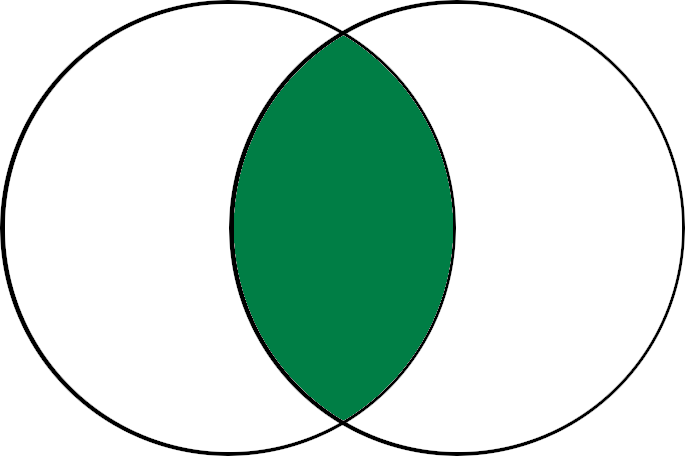
\includegraphics[width=0.3\textwidth]{figures/set_intersection.png}
      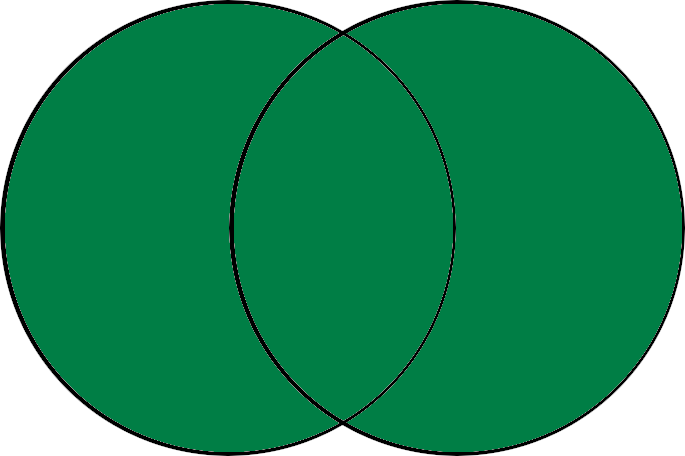
\includegraphics[width=0.3\textwidth]{figures/set_union.png}
      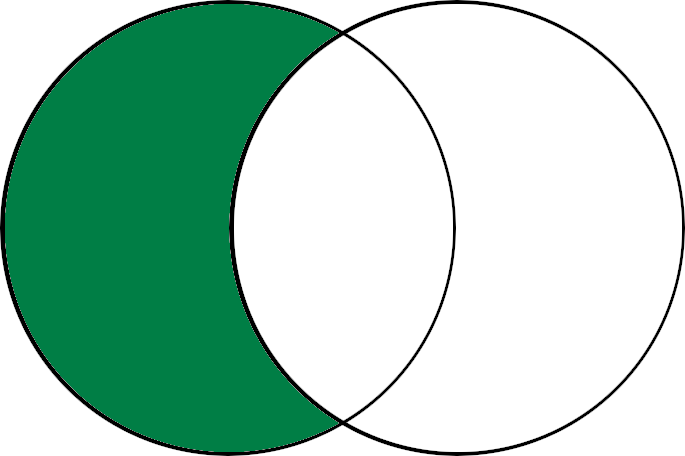
\includegraphics[width=0.3\textwidth]{figures/set_difference.png}
      
\includegraphics[width=0.3\textwidth]{figures/set_symmetric_difference.png}
    \end{multicols}
    \caption{Top Left: Intersection; Top Right: Difference;
      Bottom Left: Union; Bottom Right: Symmetric Difference}
  \end{figure}
\end{frame}

\begin{frame}[fragile]
  \frametitle{set\_intersection, set\_union, set\_difference, set\_symmetric\_difference}
  Time Complexity: $O(n)$\\
  Space Complexity: $O(n)$\\
  Usage examples:
  \begin{lstlisting}[language=C++]
std::vector<int> vec_1 = {...};
std::sort(vec_1.begin(), vec_1.end());
std::vector<int> vec_2 = {...};
std::sort(vec_2.begin(), vec_2.end());

std::vector<int> intersection;
std::set_intersection(vec_1.begin(), vec_1.end(),
  vec_2.begin(), vec_2.end(),
  std::inserter(intersection, intersection.begin()));
  \end{lstlisting}
\end{frame}

\begin{frame}[fragile]
  \frametitle{Lambdas}
  C++ 11 introduced syntax for definining functors inline:
  \begin{lstlisting}[language=C++]
auto functor = [](const int i) {
  return (i % 2) == 0;
};
  \end{lstlisting}
This is the same as:
  \begin{lstlisting}[language=C++]
struct isEvenFunctor {
  bool operator()(const int i) {
    return (i % 2) == 0;
  }
};

isEvenFunctor functor;
  \end{lstlisting}
\end{frame}

\begin{frame}[fragile]
  \frametitle{Lambda Capture Clauses}
  What if the functor needs some information which isn't passed as a parameter to operator()?
  Lambda capture clauses specify variables to be captured, eiter by value (implicitly const)
  or by reference (not const)
  \begin{lstlisting}[language=C++]
int a = 5, b = 7;
auto functor = [a, &b](const int i) {
  a += i; // ERROR: a is const
  b += i; // Okay
  return (i % 2) == 0;
};
  \end{lstlisting}
This is the same as:
  \begin{lstlisting}[language=C++]
struct isEvenFunctor {
  isEvenFunctor(int &a_, int &b_) : a(a_), b(b_) {}
  bool operator()(const int i) { ... }
  const int a;
  int &b;
} functor(a, b);
  \end{lstlisting}
\end{frame}

\begin{frame}[fragile]
  \frametitle{Bonus: ``Easy'' Parallelization}
  Just include the ``execution'' header and specify either sequenced or unsequenced parallelism
  as the first argument!
  Assuming your standard library implementation supports it...
  \begin{lstlisting}[language=C++]
#include <execution>
...
std::sort(std::execution::par,
  my_container.begin(), my_container.end());
std::reduce(std::execution::par,
  my_container.begin(), my_container.end(),
  reduction_operator);
  \end{lstlisting}
  Caveat emptor - this assumes your operator supports parallel execution.
  Operators that perform side-effects will need to appropriately guard against race conditions\\
  nvidia HPC C++ compiler (formerly PGI C++ compiler) automatically runs these on the GPU with the appropriate compiler flag
\end{frame}

\end{document}
